\documentclass[]{course-notes}


\title{Detailed \\ Sub--Assembly\\ Design}
\author[Gopsill et al.]{\normalsize James Gopsill, Rick Lupton, Geraint Owen \& Glen Mullineux}


\begin{document}

\maketitle

\section*{Abstract}

\begin{abstract}
    This document contains the course notes for the Detailed Sub-Assembly (shaft) design exercise. 
    In this exercise, we go through the full detailed analysis of a component and the specification of the associated components that will be attached to the component. 
\end{abstract}

\setcounter{tocdepth}{2}
\tableofcontents
\listoffigures
\listoftables

\section*{List of Acronyms}
\begin{acronym}[TDMA]
    \acro{PDS}{Product Design Specification}
    \acro{SYS}{Shear Yield Strength}
    \acro{TYS}{Tensile Yield Strength}
    \acro{USS}{Ultimate Shear Strength}
    \acro{UTS}{Ultimate Tensile Strength}
    \acro{YS}{Yield Strength}
\end{acronym}

\clearpage
\section{Comparing Stress and Allowable Stress}

\newthought{now armed with the calculations} for the shaft stresses and design factor, you will need to select nodes along the shaft that you feel may be critical to its operation. This is for you to decide and to discuss within your reports.

With the nodes selected, you can start to populate the excel spreadsheet that is provided. Placing the calculations within the cells enables you to quickly perform iterations of the shafts design and clearly articulate the changes to the shafts geometry. You will be submitting the final spreadsheet so we can review your calculations within the cells. Please do not alter the format of the spreadsheet. 

\begin{table}[h!]
  \caption{Spreadsheet stress model}
  \centering
  \small
  \begin{tabular}{l | c | c c c}
    \toprule
      & Node No. & 1 & 2 & 3\\
    Node Details & Units & \\
    \midrule
    Diameter \\
    Area \\
    Second Moment of Area \\
    Second Polar Moment of Area \\
    \midrule
    Forces \\
    \midrule
    Vertical \\
    Horizontal \\
    Resultant \\
    Resultant Angle \\
    \midrule
    Bending \\
    \midrule
    Vertical \\
    Horizontal \\
    Resultant \\
    Torque \\
    \midrule
    Stresses \\
    \midrule
    Direct Stress \\
    Bending Stress \\
    Torsional Stress \\
    \midrule
    Principal Stresses \\
    \midrule
    Principal Stress 1 (+) \\
    Principal Stress 2 (-) \\
    Shear Stress \\
    \midrule
    Safety Factors \\
    \midrule
    a \\
    b \\
    c \\
    d \\
    k \\
    Nu \\
    \midrule
    UTS \\
    Allowable Stress \\
    \bottomrule
  \end{tabular}
\end{table}


\clearpage
\section{Free Body Diagrams}

Free body diagrams are a method of communicating the application and direction of forces through an object. The objective is to simplify the geometry of an object to a point where one can easily see how the forces within the object interact with one another. It is also common practice to take planes in which the forces are acting to reduce the complexity of the interaction of forces further.

\cref{fig-fbd} shows an example of a loaded beam whose forces have been split in both the horizontal and vertical directions, and are reacted by two bearings. The $+$ arrow indicates our sign convention on the drawing and relative positions of the forces are also indicated.

\begin{figure*}[ht!]
  \center
  \begin{tabular}{c c}
    \subfloat[Vertical]{
    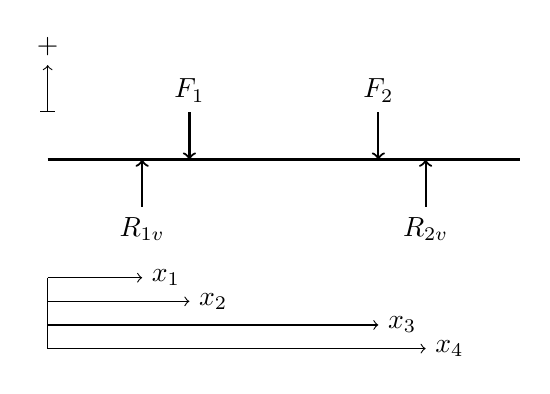
\begin{tikzpicture}[scale=6.0]
      \draw[very thick] (0,0) -- (1,0);
      
      \draw[<-, thick] (0.2,0) -- (0.2,-0.1) node[below]{$R_{1v}$};
      \draw[<-, thick] (0.8,0) -- (0.8,-0.1) node[below]{$R_{2v}$};
      
      \draw[<-, thick] (0.3,0) -- (0.3,0.1) node[above]{$F_{1}$};
      \draw[<-, thick] (0.7,0) -- (0.7,0.1) node[above]{$F_{2}$};
      
      \draw[->] (0,-0.25) -- (0.2,-0.25) node[right]{$x_1$};
      \draw[->] (0,-0.3) -- (0.3,-0.3) node[right]{$x_2$};
      \draw[->] (0,-0.35) -- (0.7,-0.35) node[right]{$x_3$};
      \draw[->] (0,-0.4) -- (0.8,-0.4) node[right]{$x_4$};
      \draw[] (0,-0.25) -- (0,-0.4);
      
      \draw[|->] (0,0.1) -- (0,0.2) node[above]{$+$};
    \end{tikzpicture}
  } &
  \subfloat[Horizontal]{
    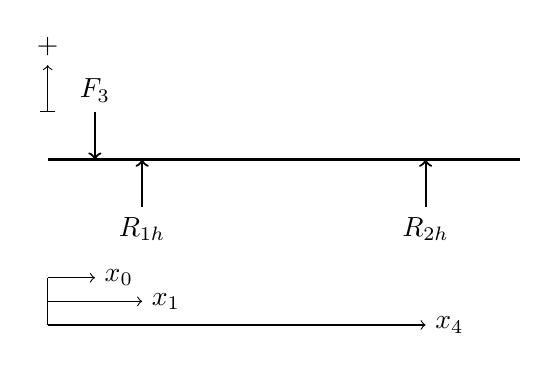
\begin{tikzpicture}[scale=6.0]
      \draw[very thick] (0,0) -- (1,0);
      
      \draw[<-, thick] (0.2,0) -- (0.2,-0.1) node[below]{$R_{1h}$};
      \draw[<-, thick] (0.8,0) -- (0.8,-0.1) node[below]{$R_{2h}$};
      
      \draw[<-, thick] (0.1,0) -- (0.1,0.1) node[above]{$F_{3}$};
      
      \draw[->] (0,-0.25) -- (0.1,-0.25) node[right]{$x_0$};
      \draw[->] (0,-0.3) -- (0.2,-0.3) node[right]{$x_1$};
      \draw[->] (0,-0.35) -- (0.8,-0.35) node[right]{$x_4$};
      \draw[] (0,-0.25) -- (0,-0.35);
      
      \draw[|->] (0,0.1) -- (0,0.2) node[above]{$+$};
    \end{tikzpicture}
  } \\
  \end{tabular}
  \vspace{1em}
  \caption{Free-body diagrams for a loaded beam}\label{fig-fbd}
\end{figure*}

Using these diagrams and information on the forces and location of the forces, one can ascertain the reactions on the bearings.

\begin{multicols}{4}
\begin{description}
    \item[$F_1$] = \SI{15}{\kilo\newton}
    \item[$F_2$] = \SI{25}{\kilo\newton}
    \item[$F_3$] = \SI{10}{\kilo\newton}
    \item[$R_{1v}$] = ?
    \item[$R_{1h}$] = ?
    \item[$R_{2v}$] = ?
    \item[$R_{2h}$] = ?
    \item[$x_0$] = \SI{0}{\metre}
    \item[$x_1$] = \SI{0.2}{\metre}
    \item[$x_2$] = \SI{0.3}{\metre}
    \item[$x_3$] = \SI{0.55}{\metre}
    \item[$x_4$] = \SI{0.6}{\metre}
\end{description}
\end{multicols}

To\marginnote{Resolving the Vertical Forces}  resolve the force vertically, we take moments about one of the bearings with the assumption that it is a static and stable system. Thus, no moment should exist about the bearing otherwise the shaft would be spinning!

Here, we have taken moments about $R_{1v}$ and from this, we can calculate the reaction force $R_{2v}$. 
\begin{align}
  \circlearrowright R_{1v} &= 0 = \SI{0.1}{\metre}(\SI{15}{\kilo\newton}) + \SI{0.35}{\metre}(\SI{25}{\kilo\newton}) - 0.4(R_{2v}) \\
  R_{2v} &= \frac{\SI{1025}{\kilo\newton\metre}}{\SI{0.4}{\metre}} = \SI{25.625}{\kilo\newton}
\end{align}

With $R_{2v}$ calculated, we can look at the balancing the forces in the vertical plane to ascertain $R_{1v}$.
\begin{align}
  R_{1v}+R_{v2}&=F_1+F_2\\
  R_{1v}+R_{v2}&=\SI{15}{\kilo\newton}+\SI{25}{\kilo\newton}\\
  R_{1v} &= \SI{40}{\kilo\newton}-\SI{25.625}{\kilo\newton} = \SI{14.375}{\kilo\newton}
\end{align}

The\marginnote{Resolving the Horizontal Forces} same process used in the horizontal direction. Taking moments about $R_{1h}$, we can find $R_{2h}$.
\begin{align}
  \circlearrowright R_{1h} &= 0 = \SI{0.2}{\metre}(\SI{10}{\kilo\newton}) + 0.4\si{\metre}(R_2) \\
  \therefore R_{2h} &=  \frac{0.2\si{\metre}}{-0.4\si{\metre}} = -5\si{\kilo\newton}
\end{align}

Again, equating the forces in the horizontal plane gives us $R_{1h}$.
\begin{align}
  R_{1h}+R_{2h}&=\SI{10}{\kilo\newton} \\
  R_{1h} &= \SI{10}{\kilo\newton} + \SI{5}{\kilo\newton} = \SI{15}{\kilo\newton}
\end{align}



\clearpage

\section{Macaulay Notation}

Macaulay Notation\footnote{N.b. This should all be familiar to you from your 1st Year Solid Mechanics.} is a method used for the structural analysis of Euler-Bernoulli beams and describes the beam forces, moments and deflection. The method is particularly useful for discontinuous and/or discrete loading scenarios as well as loadings that are uniformly distributed loads (u.d.l.) and/or uniformly varying loads (u.v.l.) over the span of a beam.

The\marginnote{Method} method starts with the Euler-Bernoulli beam theory and the relation between the deflection $w$ and bending moment $M$.

\begin{equation}
  \pm EI\frac{\text{d}^2 w}{\text{d}x^2} = M
\end{equation}

\noindent Where $E$ is the elastic modulus and $I$ is the second moment of area.

In terms of Macaulay Notation, $M$ is expressed in the form:

\begin{equation}
  M = M_1(x) + P_1\langle x-a_1\rangle^{b_1} + P_2\langle x-a_2\rangle^{b_2} + P_3\langle x-a_3\rangle^{b_3} + \ldots
\end{equation}

\noindent Where $M_1$ is the moment at the start of $x$ and $P_i\langle x-a_i\rangle^{b_i}$ representing elements along the beam that contribute to the moment. These contribute to the scenario when $x$ becomes greater than $a_i$:

\begin{equation}
  \langle x - a_i\rangle = 
  \begin{cases} 
    0 & \mathrm{if}~ x < a_i \\ 
    x - a_i & \mathrm{if}~ x > a_i 
  \end{cases}
\end{equation}

\noindent $b_i$ is determined by the type of loading that is being applied. 

For\marginnote{Shear Force} the shaft design exercise, you will be taking the shear forces and integrating them to get your bending moments for the two axes. For example, the Macaulay Notation for the Free Body Diagrams in \cref{fig-fbd} are as follows:
\begin{equation}
  S_v = R_{v1}\langle x-x_1\rangle^0 + F_{1}\langle x-x_2\rangle^0  + F_{2}\langle x-x_3\rangle^0 + R_{v2}\langle x-x_4\rangle^0
\end{equation}
\begin{equation}
  S_h = F_{3}\langle x-x_0\rangle^0 + R_{h1}\langle x-x_2\rangle^0 + R_{h2}\langle x-x_4\rangle^0
\end{equation}

From\marginnote{Shear Force Diagram} these equations, the shear force diagrams for the two axes can be generated (\cref{fig-sfd}).

\begin{figure*}[th!]
    
    \hfill{}
    \subfloat[Vertical Shear]{
        \includestandalone[width=0.4\textwidth, mode=buildnew]{03_macaulay_notation/vertical_shear}
    }
    \hfill{}
    \subfloat[Horizontal Shear]{
        \includestandalone[width=0.4\textwidth, mode=buildnew]{03_macaulay_notation/horizontal_shear}
    }
    \hfill{}
    \leavevmode\newline
    
    \hfill{}
    \subfloat[Vertical Bending]{
        \includestandalone[width=0.4\textwidth, mode=buildnew]{03_macaulay_notation/vertical_bending}
    }
    \hfill{}
    \subfloat[Horizontal Bending]{
        \includestandalone[width=0.4\textwidth, mode=buildnew]{03_macaulay_notation/horizontal_bending}
    }
    \hfill{}
    
    \vspace{2em}
    \caption{Shear force diagrams}
    \label{fig-sfd}
\end{figure*}


Having\marginnote{Bending Moment}  described the shear forces in Macaulay Notation, it is then the case of integrating and determining the constant of integration to arrive at an equation that describes the bending moment at any point through the beam.
\begin{equation}
  M_v = \int S_v = R_{v1}\langle x-x_1\rangle^1 + F_{1}\langle x-x_2\rangle^1  + F_{2}\langle x-x_3\rangle^1 + R_{v2}\langle x-x_4\rangle^1
\end{equation}
\begin{equation}
  M_h = \int S_h = F_{3}\langle x-x_0\rangle^1 + R_{h1}\langle x-x_2\rangle^1 + R_{h2}\langle x-x_4\rangle^1
\end{equation}

Using\marginnote{Bending Moment Diagram} these equations, one can obtain the bending moment diagrams for the loaded beam \pref{fig-sfd}.



\clearpage
\section{Comparing Stress and Allowable Stress}

\newthought{now armed with the calculations} for the shaft stresses and design factor, you will need to select nodes along the shaft that you feel may be critical to its operation. This is for you to decide and to discuss within your reports.

With the nodes selected, you can start to populate the excel spreadsheet that is provided. Placing the calculations within the cells enables you to quickly perform iterations of the shafts design and clearly articulate the changes to the shafts geometry. You will be submitting the final spreadsheet so we can review your calculations within the cells. Please do not alter the format of the spreadsheet. 

\begin{table}[h!]
  \caption{Spreadsheet stress model}
  \centering
  \small
  \begin{tabular}{l | c | c c c}
    \toprule
      & Node No. & 1 & 2 & 3\\
    Node Details & Units & \\
    \midrule
    Diameter \\
    Area \\
    Second Moment of Area \\
    Second Polar Moment of Area \\
    \midrule
    Forces \\
    \midrule
    Vertical \\
    Horizontal \\
    Resultant \\
    Resultant Angle \\
    \midrule
    Bending \\
    \midrule
    Vertical \\
    Horizontal \\
    Resultant \\
    Torque \\
    \midrule
    Stresses \\
    \midrule
    Direct Stress \\
    Bending Stress \\
    Torsional Stress \\
    \midrule
    Principal Stresses \\
    \midrule
    Principal Stress 1 (+) \\
    Principal Stress 2 (-) \\
    Shear Stress \\
    \midrule
    Safety Factors \\
    \midrule
    a \\
    b \\
    c \\
    d \\
    k \\
    Nu \\
    \midrule
    UTS \\
    Allowable Stress \\
    \bottomrule
  \end{tabular}
\end{table}


\clearpage
\section{Design Factor}\label{sec:DF}

The Design Factor (\(N_u\)/\(N_y\)) is used to obtain an ``allowable'' or ``working'' stress for design calculations. The design factor may be based on a number of failure modes, such as \ac{UTS} or endurance limit.

When considering the \ac{UTS}, the Design Factor (\(N_u\)) is:

\begin{equation}
    N_u = a.b.c.d.k 
\end{equation}

And the allowable stress is calculated by:

\begin{equation}
    \text{Allowable Stress} = \frac{S_\text{UTS}}{N_u}
\end{equation}

When considering the \acf{YS}, the Design Factor (\(N_y\)) is:

\begin{equation}
    N_y = b.c.d.k
\end{equation}

And the allowable stress is calculated by:

\begin{equation}
    \text{Allowable Stress} = \frac{S_\text{y}}{N_y} 
\end{equation}

The five factors \(a\), \(b\), \(c\), \(d\) and \(k\) ensure that we consider the following in our calculations: 

\begin{description}
    \item[a] ratio between \ac{UTS} and \ac{YS} for your material
    \item[b] fatigue factor
    \item[c] shock factor
    \item[d] factor of safety (Pugsley's Method)
    \item[k] stress concentration factor
\end{description}

The\marginnote{a: UTS / YS ratio} ratio of the ultimate strength of the material to its yield strength (sometimes the elastic limit). If the yield strength is not known then this factor is used to estimate what it would be:

\begin{description}
    \item[\(a=2\)] for ductile material
    \item[\(a=1.5\)] for heat treated and tempered alloys
\end{description}

For cast iron, which has no real elastic limit, failure occurs suddenly at the ultimate tensile strength, and there is no sense in applying this factor at all.

The\marginnote{b: Fatigue Factor} fatigue factor can be calculated using the Goodman Criterion but in general and for the purpose of this exercise, you should consider two scenarios:

%used to quantify the interaction of mean and alternating stresses on the fatigue life of a material.

%\begin{equation}
%  \sigma_\text{a} = \sigma_\text{fat}\times\left(1-\frac{\sigma_\text{m}}{\sigma_\text{ts}}\right).
%\end{equation}

%\noindent Where $\sigma_\text{a}$ is the alternating stress, $\sigma_\text{m}$ is the mean stress, $\sigma_\text{fat}$ is the fatigue limit for completely reversed loading, and $\sigma_\text{ts}$ is the ultimate tensile strength of the material. But in general and for the purpose of this exercise, you should consider two scenarios:

\begin{description}
    \item[\(b=1\)] for a dead load, or a single-plane load varying between 0 and a maximum.
    \item[\(b=1.5\)] for a load that varies between tension and compression
\end{description}

The\marginnote{c: Shock Factor} dynamic forces imposed by shock loading can be many times the static loads that a shaft is designed towards. If there is potential for a shock load, a safety factor should be included to account. Again, you should consider two cases.

\begin{description}
    \item[\(c=1\)] when loads are gradually applied
    \item[\(c=2\)] when loads are suddenly applied
\end{description}

To investigate the shock loads in detail, analysis of the elongation and energy absorption capability of material and geometry would be required.

The\marginnote{d: ``Factor of Safety''} ``Factor of Safety'' or uncertainty factor can be considered the ``real'' safety factor. 

If all the other factors (a,b,c,k) are properly computer and accounted for, and the ``design factor'' made equal to their product, the design will still have nor margin of safety to allow for unexpected variation in load or material quality. It may be on the point of failure and these factors may be indeterminate, or extremely complex, or uncertain.

The factor d provide for these conditions, The value taken for d will be dependent on the judgement of the designer, but will include the consideration of the following:

\begin{enumerate}
    \item Degree of accuracy of stress computations \emph{(I.e.\ the reliance that can be placed on the estimation of and the assumptions made in calculating the stresses.)}
    \item Degree of reliability of the material \emph{I.e.\ the conformance to specification of the material chosen and the property chosen to represent the behaviour of the material under the specified loading.}
    \item Degree of uncertainty of loading \emph{I.e.\ How reliable the load specification is both in terms of magnitude, point of application, distribution of loading and inclusion of other loads such as handling, transportation etc.}
    \item Degree of reliability of specification \emph{I.e.\ How reliable the ``specification'' is in terms of defining the function etc.}
    \item Initial stresses \emph{I.e.\ Presence of residual stresses associated with manufacture, forming or assembly etc.}
    \item Reliability of manufacture \emph{I.e.\ Variability of heat treatments, surface finishes, dimensional tolerances etc.}
    \item Indeterminate or unexpected loads \emph{I.e.\ Errors in handling, changes in loading due to wear of critical parts etc.}
    \item Operating environment \emph{I.e.\ Ambient temperature (high or low), corrosion etc.}
    \item Consequences of failure \emph{I.e.\ Danger to life, ease of repair, cost of failure etc.}
\end{enumerate}

A safety factor may be defined by a Code of Practice, Company Policy, experience of designer. Codes of Practice specifying Safety Factors are often associated with specialised industries for products such as boilers, buildings etc. Companies dealing with specialised products frequently have their own specified factors of safety. Caution should be exercised where the design differs from the ``norm''. Experienced designers will often have developed their own safety factors for application to their design speciality.


In\marginnote{Calculating d using Pugsley's Method} 1966, Pugsley \mycite{howard1967} devised a general methodology for determining the safety factor, which takes the manufacturing, operational characteristics, and seriousness of failure into account\footnote{For more information on Safety Factors please see \cref{appendix-safety}}.

\begin{equation}
    d = X.Y
\end{equation}

\begin{description}
    \item[\(X\)] is chosen based on three factors related to manufacture and operation.
    \item[\(Y\)] is chosen based on seriousness of failure related to personnel and to economic impact.
\end{description}

To calculate the value of \(X\), one has to determine the quality of the component in three areas:

\begin{description}
    \item[A] Materials, workshop, inspection and manufacture
    \item[B] Loading and control over it
    \item[C] Quality of assessment of strength, analysis methods and accuracy
\end{description}

Each are scored as either Very Good (VG), Good (G), Fair (F) or Poor (P). Using these scores, the value for \(X\) can be calculated using \cref{tbl-pugsley-x}.

\begin{table}[h!]
  \caption{Calculating $X$}\label{tbl-pugsley-x}
  \center{}
  \begin{tabular}{l c | c c c c}
    \toprule
    & B = & VG & G & F & P \\
    A = & C = & & & & \\
    \midrule
    VG & VG & 1.1 & 1.3 & 1.5 & 1.7 \\
    VG & G & 1.2 & 1.45 & 1.7 & 1.95 \\
    VG & F & 1.3 & 1.6 & 1.9 & 2.2 \\
    VG & P & 1.4 & 1.75 & 2.1 & 2.45 \\
    \midrule
    G & VG & 1.4 & 1.55 & 1.8 & 2.05 \\
    G & G & 1.45 & 1.75 & 2.05 & 2.35 \\
    G & F & 1.6 & 1.95 & 2.3 & 2.65 \\
    G & P & 1.75 & 2.15 & 2.55 & 2.95 \\
    \midrule
    F & VG & 1.5 & 1.8 & 2.1 & 2.4 \\
    F & G & 1.7 & 2.05 & 2.4 & 2.75 \\
    F & F & 1.9 & 2.3 & 2.7 & 3.1 \\
    F & P & 2.1 & 2.55 & 3.00 & 3.45 \\
    \midrule
    P & VG & 1.7 & 2.15 & 2.4 & 2.75 \\
    P & G & 1.95 & 2.35 & 2.75 & 3.15 \\
    P & F & 2.2 & 2.65 & 3.1 & 3.55 \\
    P & P & 2.45 & 2.95 & 3.45 & 3.95 \\
    \bottomrule
  \end{tabular}
\end{table}

To calculate the value of \(Y\), one has to assess the potential impact of the failing with respect to two areas:

\begin{description}
  \item[D] Seriousness of danger to personnel
  \item[E] Seriousness of economic consequences
\end{description}

These are scores Not Serious, Serious and Very Serious. Table~\ref{tbl-pugsley-y} is then used to look-up the respective \(Y\) value.

\begin{table}
  \caption{Calculating $Y$}\label{tbl-pugsley-y}
  \center{}
  \begin{tabular}{c c c c}
    \toprule
    D = & Not Serious & Serious & Very Serious \\
    E = & & & \\
    \midrule
    Not Serious & 1 & 1.2 & 1.4 \\
    Serious & 1.1 & 1.3 & 1.5 \\
    Very Serious & 1.2 & 1.4 & 1.6 \\
    \bottomrule
  \end{tabular}
\end{table}

This\marginnote{k: Stress Concentration Factor} allows for the fact that there may be sudden changes in the geometry of a part. An example is fillets that provide places where localised stresses are higher than those determined by simple stress analysis. A wealth of empirical and analytical studies have been performed to determine the stress concentration factors for features, such as fillets and circlip grooves (\cref{fig-stress-fillet,fig-stress-circlip}, respectively). 

\begin{figure*}[t!]
  
    \hfill{}
    \subfloat[Bending]{
        \includestandalone[width=0.45\textwidth]{05_design_factor/fillet-bending}
        %\includegraphics[width=0.45\textwidth]{05_design_factor/fillet-bending.png}
    }
    \hfill{}
    \subfloat[Torsion]{
        \includestandalone[width=0.45\textwidth]{05_design_factor/fillet-torsion}
        % \includegraphics[width=0.45\textwidth]{05_design_factor/fillet-torsion.png}
    }
    \hfill{}
    
    \vspace{1em}
    \caption{Fillet stress concentration factors for shafts}\label{fig-stress-fillet}
\end{figure*}

\begin{figure*}[t]
    
    \hfill{}
    \subfloat[Bending]{
        \includestandalone[width=0.45\textwidth]{05_design_factor/circlip-groove-bending}
        %\includegraphics[width=0.45\textwidth]{05_design_factor/circlip-groove-bending.png}
    }
    \hfill{}
    \subfloat[Torsion]{
        \includestandalone[width=0.45\textwidth]{05_design_factor/circlip-groove-torsion}
        %\includegraphics[width=0.45\textwidth]{05_design_factor/circlip-groove-torsion.png}
    }
    \hfill{}
    
    \vspace{1em}
    \caption{Circlip stress concentration factors for shafts}\label{fig-stress-circlip}
\end{figure*}



\clearpage
\section{Comparing Stress and Allowable Stress}

\newthought{now armed with the calculations} for the shaft stresses and design factor, you will need to select nodes along the shaft that you feel may be critical to its operation. This is for you to decide and to discuss within your reports.

With the nodes selected, you can start to populate the excel spreadsheet that is provided. Placing the calculations within the cells enables you to quickly perform iterations of the shafts design and clearly articulate the changes to the shafts geometry. You will be submitting the final spreadsheet so we can review your calculations within the cells. Please do not alter the format of the spreadsheet. 

\begin{table}[h!]
  \caption{Spreadsheet stress model}
  \centering
  \small
  \begin{tabular}{l | c | c c c}
    \toprule
      & Node No. & 1 & 2 & 3\\
    Node Details & Units & \\
    \midrule
    Diameter \\
    Area \\
    Second Moment of Area \\
    Second Polar Moment of Area \\
    \midrule
    Forces \\
    \midrule
    Vertical \\
    Horizontal \\
    Resultant \\
    Resultant Angle \\
    \midrule
    Bending \\
    \midrule
    Vertical \\
    Horizontal \\
    Resultant \\
    Torque \\
    \midrule
    Stresses \\
    \midrule
    Direct Stress \\
    Bending Stress \\
    Torsional Stress \\
    \midrule
    Principal Stresses \\
    \midrule
    Principal Stress 1 (+) \\
    Principal Stress 2 (-) \\
    Shear Stress \\
    \midrule
    Safety Factors \\
    \midrule
    a \\
    b \\
    c \\
    d \\
    k \\
    Nu \\
    \midrule
    UTS \\
    Allowable Stress \\
    \bottomrule
  \end{tabular}
\end{table}




\clearpage
\section{Transmission Selection}

As part of your design, you will need to select the type of transmission and subsequent specification of your chosen transmission. You will need to do some research on the types of transmission to be able to present a reasoned argument for your selection. This will be followed by the steps taken to select an initial specification of transmission. In this document, we will take your through the selection of a chain transmission. For other transmission types, you will have to look up the relevant guides and processes. Do not let this put you off though as the steps are fairly similar.

\subsection{Transmission Types}

\begin{framed}
    \vspace{1cm}
    \begin{center}
        \Large
        -- Own Research \& Lectures --
    \end{center}
    \vspace{1cm}
\end{framed}

\subsection{Selecting a Chain Drive}

The following selection of a chain drive uses Renold's Chain Guide\footnote{Acknowledgements to the Renold Chain Guide}. Other chain companies will have similar processes and it is important to follow the appropriate companies' process when selecting your transmission.

\subsubsection{Features \& Considerations}

An\marginnote{Centre Distance}  incorrect centre distance leads to a higher wear rate and slack chain, which introduces further inefficiencies into the system. % Centre distances that are smaller than nominal can be attained through the use of a chain tensioner.

When\marginnote{Polygonal Action} the driving sprocket of a chain drive runs at constant speed, the speed of the chain itself is not constant but is subject to periodic fluctuations. This fluctuation, which is caused by the fact that the chain when wrapped on a sprocket forms a polygon rather than a circle, is known as polygonal action \mycite{mahalingam1958}.

One effect of polygonal action is to produce a periodic variation in the velocity ratio of the drive, and if the frequency of this variation coincides with a resonant frequency of the system, large stresses may occur. At high chain speeds the effects of impact are very complex; each impact sets up a train of travelling waves which, after reflection at the sprockets, combine with the next train and so on.

\cref{fig-cyclic-speed-variation} highlights that polygonal actions' effect increases considerably as one decreases the no.\ of sprocket teeth below 19. Hence, Renold recommends that sprockets should have a minimum of 19 teeth to avoid the effect of polygonal action. If lower teeth are required, then an additional factor is applied when selecting a chain, which reduces the maximum rated speed of the chain.

\begin{marginfigure}
    \centering
    \includegraphics[width=\textwidth]{07_transmission_selection/polygonal-action.png}
    \caption[Cyclic speed variation due to polygonal action]{Cyclic speed variation due to polygonal action \cite[][p.24]{renoldchain}}
    \label{fig-cyclic-speed-variation}
\end{marginfigure}

It\marginnote{cranked link} is always best practice and desirable to have a chain with an even number of links. However, when there is a case that requires an odd linked chain, cranked links are used to form the chain loop. \cref{fig-cranked-link} shows an example of a cranked link within a chain. The link has a natural kink in the profile to allow it to connect to the next link in the chain. This inherently places additional stress concentrations within the component and thus, is not recommended for high load and/or speed chain drives.


\begin{marginfigure}
    \centering
    \includegraphics[width=\textwidth]{07_transmission_selection/cranked-link.png}
    \caption[Cranked link]{Cranked link~\cite
    [][p.11]{renoldchain}}
    \label{fig-cranked-link}
\end{marginfigure}

\subsubsection{Selection Process}

The selection process for a Renold chain is as follows. The prerequisites for the process is that you know the torque and sprocket speeds that you wish to run at.

The\marginnote{Selection Power (\(P_s\))} selection power is calculated by multiplying the power you wish to transmit (\(P_s\)) by two safety factors \(f_1\) and \(f_2\).

\begin{equation}
  P_s = f_1f_2P_t
\end{equation}

\noindent Where:

\begin{description}
  \item[\(f_1\)] Safety factor depending on your operation and can be found using chart 2 on p.28 of the Renold catalogue
  \item[\(f_2\)] Adjustment factor is your are using the non-recommended number of driving sprocket teeth. \(f_2=\frac{19}{\text{No. of teeth on driving}}\)
\end{description}

With\marginnote{Selecting a Suitable Chain Pitch} the selection power determined and the driver sprocket speed known, one can determine the chain pitch using \cref{fig-chain-pitch}. These rating charts have been created from years of empirical testing and theoretical modelling by the chain companies, and dictate the safe operating windows for their selection of chains.

\begin{figure}[h!]
    \centering
    \includegraphics[width=0.9\textwidth]{07_transmission_selection/chain-pitch.png}
    \caption[Chain pitch selection chart]{Chain pitch selection chart \cite[][p.31]{renoldchain}}
    \label{fig-chain-pitch}
\end{figure}

After\marginnote{Select Chain and Sprockets} selecting the chain pitch, you can go through the catalogue to find the drive and driven sprockets that will give you the required (or as near as possible) ratio for your design.

Having\marginnote{Chain Links and Centre Distance} the chain pitch and sprockets selected, the centre distance

\begin{equation}
    L = \frac{Z_1+Z_2}{2}+\frac{2C_1}{P}+\frac{P{\left(\frac{Z_2-Z_1}{2\pi}\right)}^2}{C_1}
\end{equation}

\noindent{} Where:

\begin{description}
    \item[\(Z_1\)] Number of driving teeth
    \item[\(Z_2\)] Number of driven teeth
    \item[\(C_1\)] Approximate desired centre distance
    \item[\(P\)] Chain pitch
    \item[\(L\)] Number of chain links
\end{description}

Once calculated, you then round to the nearest even integer and use this to calculate your centre distance \(C\).

\begin{equation}
    C=\frac{P}{8}
    \left[
    2L-Z_2-Z_1 
    +
    \sqrt{ 
    {\left(2L-Z_2-z_1\right)}^2 - \left(\frac{\pi}{3.88}\left(Z_2-Z_1\right)^2\right)
    }
    \right]
\end{equation}

\subsubsection{Chain Example}

Select a chain and sprocket to transmit \SI{2}{\kilo\watt} of power at \SI{20}{rpm}. A ratio of 1:2 is required, driven by an electric motor with moderate shocks expected from the load. Space is highly limited.

Using\marginnote{Determining \(f_1\) and \(f_2\)} Chart 2 on p.28 of the Renold catalogue, we identify that \(f_1=1.4\) for our context and we will also use the recommended number of teeth on the driving sprocket (19), which makes \(f_2=1\). Therefore, the selection power \(P_s\) becomes:

\begin{equation}
    P_s = f_1f_2P_t = 2\si{\kilo\watt}\times1.4\times1=2.8\si{\kilo\watt}
\end{equation}

Using\marginnote{Chain Pitch} \cref{fig-chain-pitch}, we can find the chain pitches that are suitable for our application. The potential pitches are:

\begin{itemize}
    \item \SI{38.10}{\milli\metre} simplex
    \item \SI{31.75}{\milli\metre} duplex
    \item \SI{25.40}{\milli\metre} triplex
\end{itemize}

For\marginnote{Chain and Sprocket Selection} this example, we will select the triplex as our requirement is to have a compact solution. Now it is just a case of looking in the tables to find a sprocket set (Renolds, p.75) that will provide us with a ratio that provides us with the closest match in terms of our desired ratio, and a triplex chain (Renolds, p.25).

\begin{description}
    \item[Chain] 12B-3
    \item[Driving Sprocket] 16B1/19T
    \item[Driven Sprocket] 16B1/38T
\end{description}

Now\marginnote{Chain Links} we have the sprockets and chain selected, it is then a simple case of using their specifications to determine the number of links:

\begin{equation}
    L = 
    \frac{19+38}{2}
    +
    \frac{2\times571.5}{19.05}+\frac{19.05{\left(\frac{38-19}{2\pi}\right)}^2}{571.5} = 88.6
\end{equation}

Rounding this up to the nearest even integer gives us \(L=90\).

The\marginnote{Centre Distance} final calculation is to determine the centre distance:

% https://www.sharelatex.com/learn/Aligning_equations_with_amsmath
\begin{equation}
\begin{split}
    C & = \frac{19.05}{8}
    \left[
    2(90)-38-19 
    +
    \sqrt{ 
    {\left(2(90)-38-19\right)}^2 - \left(\frac{\pi}{3.88}\left(38-19\right)^2\right)
    }
    \right] 
    \\ & = \SI{583}{\milli\metre}
\end{split}
\end{equation}

\subsection{Selecting a vee-belt or tooth belt}

\begin{framed}
    \vspace{1cm}
    \begin{center}
        \Large
        -- Own Research \& Lectures --
    \end{center}
    \vspace{1cm}
\end{framed}



\clearpage
\section{Bearing Selection}

This section details the process in selecting bearings from the SKF catalogue. However, it is up to you to do your own research and attend the lectures to understand and determine the most appropriate bearings for your design problem.

\subsection{Bearing Types and Locating Bearings}

\begin{framed}
    \vspace{1cm}
    \begin{center}
        \Large
        -- Own Research \& Lectures --
    \end{center}
    \vspace{1cm}
\end{framed}

%\marginnote{Deep-Groove Ball \\ 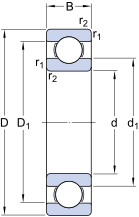
\includegraphics[width=0.06\textwidth]{single-deep-groove-ball-bearing.png}}

%\vspace{3cm}

%\marginnote{Angular Contact Bearing \\ 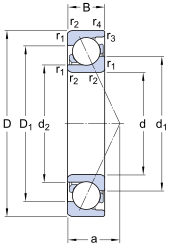
\includegraphics[width=0.07\textwidth]{angular-contact-bearing.png}}

%\vspace{3cm}

%\marginnote{Taper Roller \\ 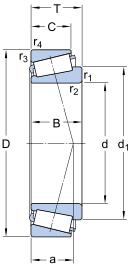
\includegraphics[width=0.07\textwidth]{taper-bearing.png}}

%\vspace{3cm}

%\marginnote{Cylindrical Roller \\ 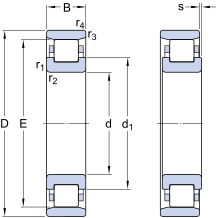
\includegraphics[width=0.07\textwidth]{cylindrical-roller-bearing.png}}

%\vspace{3cm}

%\marginnote{Y-Bearing \\ 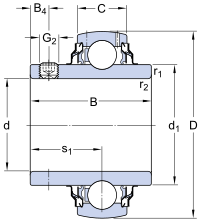
\includegraphics[width=0.2\textwidth]{y-bearing.png}}

%\vspace{3cm}

%\subsection{Locating Bearings}

%\begin{framed}
%  \vspace{2cm}
%    \begin{center}
%      {\fontsize{50}{60}\selectfont \faQuestion{}}\\
%      Research Required
%    \end{center}
%  \vspace{2cm}
%\end{framed}

%\marginnote{\it float}

%\marginnote{\it stepped shaft}

%\marginnote{\it fillet radius}

%\marginnote{\it spacer}

%\marginnote{\it undercut}

%\marginnote{\it pre-load}

\subsection{Bearing Calculations} 

Once you have decided upon the bearing arrangement for your shaft, we can use SKF's bearing selection process to determine the size of bearing that is required. Manufacturers often provide a selection process for their bearings, which they have developed over years of experience in designing and manufacturing their products. The SKF process requires us to determines the basic dynamic \(C\) and static \(C_0\) load ratings that we require for our bearings, which are in accordance of ISO 281:2007 and ISO 76:2006, respectively.


Lets\marginnote{Basic Static Load Rating (\(C_0\))}  start with calculating the basic static load rating for a bearing. This can be calculated using Equation~(\ref{equ-basic-load-rating}) and is where the equivalent static load \(P_0\) is multiplied by a safety factor \(S_0\).

\begin{equation}
    C_0 = P_0 S_0
    \label{equ-basic-load-rating}
\end{equation}

Thus, we need to know both \(P_0\) and \(S_0\).

The\marginnote{Equivalent Static Load (\(P_0\))} calculation for \(P_0\) is dependent upon the type of bearing you're looking to selecting. In the case of a deep-groove ball bearing, \(P_0\) is calculated by:

\begin{equation}
    \text{Calculate } P_0 = 0.6F_r+0.5F_a \text{ then if, } P_0 \le F_r \text{ we set, }P_0 = F_r
\end{equation}

This\marginnote{Safety Factor (\(S_0\))} is then multiplied by the Safety Factor (\(S_0\)), which is selected based on the shafts operating condition.

\begin{itemize}
    \item 0.5 for smooth and shock free
    \item 1.0 for normal
    \item 1.5 for shock and vibration
\end{itemize}

Now\marginnote{Basic Dynamic Load Rating (\(C\))}  we have calculated \(C_0\), we can move onto the basic dynamic load raring (\(C\)), which is calculated through the re-arrangement of the following equation:

\begin{equation}
    L_{10} = \left(\frac{C}{P}\right)^p
    \label{equ-bearing-life}
\end{equation}

\noindent{} Where:

\begin{description}
    \item[\(L_{10}\)] Is the number of revolutions at constant speed that 90\% of bearings tested will complete or exceed before the first evidence of failure develops. This is usually standardised to 1,000,000 cycles in accordance with ISO 281:2007.
    \item[\(C\)] basic dynamic loading rating (\si{\kilo\newton})
    \item[\(P\)] equivalent dynamic bearing load (\si{\kilo\newton})
    \item[\(p\)] bearing factor
    \begin{itemize}
        \item Ball Bearing, \(p=3\)
        \item Roller Bearing, \(p=\frac{10}{3}\)
    \end{itemize}
\end{description}

Thus, to calculate \(C\), we need to know both \(L_{10}\) and \(P\).

To\marginnote{life rating (\(L_{10}\))} determine the life rating (in cycles),

\begin{equation}
    L_{10} = \text{Hours of Operation} \times \text{rpm} \times 60
\end{equation}

With\marginnote{Equivalent Dynamic Bearing Load (\(P\))} \(L_{10}\) now known, we can focus our attention onto \(P\). The calculation for \(P\) is dependent upon the type of bearing you're looking to selecting. In the case of a deep-groove ball bearing (SKF p.316).

\begin{equation}
    P = XF_r + YF_a
\end{equation}

To determine the coefficients \(X\) and \(Y\), we need to find the calculation factors \(f_0\) and \(e\).

From the catalogue, \(f_0\) is calculated using:

\begin{equation}
    f_0 = \frac{F_a}{C_0}
\end{equation}

And \(e\) can be found using the look-up table on page XX in the catalogue. In this case, \(e=0.22\). With these values, we can then decide on, which equivalent dynamic bearing load calculation we require (SKF p.316). One example is:

\begin{equation}
    \text{if, }\frac{F_a}{F_e}\le e \Rightarrow P=F_r \text{ else, } \frac{F_a}{F_e}\ge e \Rightarrow P=XF_r+YF_a
\end{equation}

Once we have \(P\), we can calculate \(C\) be re-arranging the life rating equation (\cref{equ-bearing-life}). 

\begin{equation}
    \sqrt[p]{L_{10}}\times P = C
\end{equation} 

With\marginnote{Finding a Bearing} \(C_0\) and \(C\) calculated, it is then just a case of looking through the bearing tables and finding a bearing that meets these criteria.

\subsection{Example: Deep Groove Ball Bearing Selection}

A deep groove ball bearing is needed to support a \SI{15}{\kilo\newton} radial and \SI{3}{\kilo\newton} axial loading rotating at \SI{30}{rpm}, on a shaft of \SI{30}{\milli\metre} diameter. The bearing will operate in a smooth-running environment without shock loading, and must be reliable for \SI{5000}{\hour} of operation.

From this description, we can quickly ascertain that:

\begin{itemize}
    \item Deep Groove Ball. Therefore, \(p=3\)
    \item Running speed \(\ge \SI{10}{rpm}\). Therefore, the dynamic load rating is required \(P=XF_r+YF_a\)
    \item Smooth running, vibration free and low shock loading. Therefore, the safety factor \(S_0\) is 1.
    \item \(L_{10} = 5000 \times 60 \times 30 = 9,000,000\) cycles 
\end{itemize}

\marginnote{Equivalent Static Load (\(P_0\))} Using the SKF catalogue, the equivalent static bearing load is given by:

\begin{equation}
    P_0 = 0.6F_r+0.5F_a \text{ then if, } P_0 \le F_r \text{ we set, }P_0 = F_r
\end{equation}

\noindent{} Hence, for this case, \(P_0\) is:

\begin{equation}
    P_0=0.6F_r+0.5F_a = 0.6\times\SI{15}{\kilo\newton} + 0.5\times\SI{3}{\kilo\newton} = \SI{10.5}{\kilo\newton}
\end{equation}

\noindent{} As \(P_0 \le F_r \), we set \(P_0 = F_r = 15\si{\kilo\newton} \).

Now\marginnote{Basic Static Load Rating (\(C_0\))} we can calculate our static load rating \(C_0\) using:

\begin{equation}
    C_0=P_0S_0
\end{equation}

\noindent{} And for our case, \(C_0\) becomes:

\begin{equation}
    C_0= \SI{15}{\kilo\newton} \times 1 = \SI{15}{\kilo\newton}
\end{equation}


Having\marginnote{Equivalent Dynamic Load (\(P\))} calculated \(C_0\), we can move onto calculating the equivalent dynamic load \(P\) so that we can attain the basic dynamic load rating \(C\):

\begin{equation}
    P = XF_r + YF_a
\end{equation}

To determine the coefficients \(X\) and \(Y\), we need to find the calculation factors \(f_0\) and \(e\).

From the catalogue, \(f_0\) is calculated using:

\begin{equation}
    f_0 = \frac{F_a}{C_0} = \frac{3\si{\kilo\newton}}{15\si{\kilo\newton}} = 0.2
\end{equation}

And \(e\) can be found using the look-up table on p.315 in the catalogue. In this case, \(e=0.22\). With these values, we can then decide on, which equivalent dynamic bearing load calculation we require (SKF p.316). 

\begin{equation}
    \text{if, }\frac{F_a}{F_r}\le e \Rightarrow P=F_r \text{ else, } \frac{F_a}{F_r}\ge e \Rightarrow P=XF_r+YF_a
\end{equation}

Therefore, in our case:

\begin{equation}
    \frac{F_a}{F_r}=\frac{3\si{\kilo\newton}}{15\si{\kilo\newton}}=0.2
\end{equation}

\noindent{} and this value is \(\le e\). Thus, 

\begin{equation}
    P=F_r=15\si{\kilo\newton}
\end{equation}

Now\marginnote{Equivalent Dynamic Load Rating (\(C\))} we have all the information we need to determine the equivalent dynamic load rating \(C\) by re-arranging the life rating equation (Equation~\ref{equ-bearing-life}). 

\begin{equation}
    \sqrt[p]{L_{10}}\times P = C = \SI{31.2}{\kilo\newton}
\end{equation}

Now looking through the available bearings in the catalogue and knowing we have to fit onto a \SI{30}{\milli\metre} shaft, two bearings are potentially suitable:

\begin{itemize}
    \item 6306 ETN9
    \item 6406
\end{itemize}

Looking into more detail of the designations of the bearings reveals that ETN9 means that the bearing is reinforced. This is likely to be an over-specification for our application. Therefore, we shall select 6406.

%\subsection{Bearing Selection -- Roller Bearing Example}

%A locating roller bearing is needed to support a 60\si{\kilo\newton} radial and 25\si{\kilo\newton} axial loading rotating at 100\si{rpm}, on a shaft of 75\si{\milli\metre} diameter. The bearing will operate in a normal environment, and must be reliable for 11,000\si{\hour} of operation.

%\begin{itemize}
%  \item Roller. Therefore, \(p=\frac{10}{3}\)
%  \item Running speed \(\ge 10\si{rpm}\). Therefore, the dynamic load rating is required.
%  \item Normal running environment. Therefore, the safety factor \(S_0\) is 1.
%  \item \(L_{10} = 11,000 \times 60 \times 100 = 66,000,000\) cycles 
%\end{itemize}

%\marginnote{Basic Static Load Rating} [TO DO]

%\marginnote{Equivalent Dynamic Load \(P\)} Looking through the SKF catalogue, we identify the equation for \(P\) for locating bearings (p.594).

%\begin{equation}
%\text{If } \frac{F_a}{F_r} \leq e \text{ then } P=F_r \text{ else } P=0.92F_r+YF_a
%\end{equation}

%\begin{equation}
%  \frac{F_a}{F_r}=\frac{25\si{\kilo\newton}}{60\si{\kilo\newton}} = 0.417 > e
%\end{equation}

%To determine \(Y\), we look up the value in the respective SKF table (p.593). In this case, \(Y=0.6\). Thus, \(P\) becomes:

%\begin{equation}
%  P=0.92F_r+0.6F_a=70.2\si{\kilo\newton}
%\end{equation} 

%\marginnote{Basic Dynamic Load Rating \(C\)} Now we have \(P\), we can calculate the basic dynamic load rating \(C\).

%\begin{equation}
%  \sqrt[p]{L_{10}}\times P = C = \sqrt[\frac{10}{3}]{66,0000,000}\times 70,200=246\si{\kilo\newton}
%\end{equation}


%Looking through the SKF tables, we can find a range of suitable bearings with NUP designated bearings able to take axial loads. Focusing on these bearings, two options are available to us:

%\begin{itemize}
%  \item NUP 135 ECP
%  \item NUP 2135 ECP
%\end{itemize}


\clearpage
\section{Comparing Stress and Allowable Stress}

\newthought{now armed with the calculations} for the shaft stresses and design factor, you will need to select nodes along the shaft that you feel may be critical to its operation. This is for you to decide and to discuss within your reports.

With the nodes selected, you can start to populate the excel spreadsheet that is provided. Placing the calculations within the cells enables you to quickly perform iterations of the shafts design and clearly articulate the changes to the shafts geometry. You will be submitting the final spreadsheet so we can review your calculations within the cells. Please do not alter the format of the spreadsheet. 

\begin{table}[h!]
  \caption{Spreadsheet stress model}
  \centering
  \small
  \begin{tabular}{l | c | c c c}
    \toprule
      & Node No. & 1 & 2 & 3\\
    Node Details & Units & \\
    \midrule
    Diameter \\
    Area \\
    Second Moment of Area \\
    Second Polar Moment of Area \\
    \midrule
    Forces \\
    \midrule
    Vertical \\
    Horizontal \\
    Resultant \\
    Resultant Angle \\
    \midrule
    Bending \\
    \midrule
    Vertical \\
    Horizontal \\
    Resultant \\
    Torque \\
    \midrule
    Stresses \\
    \midrule
    Direct Stress \\
    Bending Stress \\
    Torsional Stress \\
    \midrule
    Principal Stresses \\
    \midrule
    Principal Stress 1 (+) \\
    Principal Stress 2 (-) \\
    Shear Stress \\
    \midrule
    Safety Factors \\
    \midrule
    a \\
    b \\
    c \\
    d \\
    k \\
    Nu \\
    \midrule
    UTS \\
    Allowable Stress \\
    \bottomrule
  \end{tabular}
\end{table}



\clearpage

\printbibliography[]

%\bibliography{citations}
%\bibliographystyle{plainnat}
%\bibliographystyle{plain}

\appendix

\clearpage
\section{Comparing Stress and Allowable Stress}

\newthought{now armed with the calculations} for the shaft stresses and design factor, you will need to select nodes along the shaft that you feel may be critical to its operation. This is for you to decide and to discuss within your reports.

With the nodes selected, you can start to populate the excel spreadsheet that is provided. Placing the calculations within the cells enables you to quickly perform iterations of the shafts design and clearly articulate the changes to the shafts geometry. You will be submitting the final spreadsheet so we can review your calculations within the cells. Please do not alter the format of the spreadsheet. 

\begin{table}[h!]
  \caption{Spreadsheet stress model}
  \centering
  \small
  \begin{tabular}{l | c | c c c}
    \toprule
      & Node No. & 1 & 2 & 3\\
    Node Details & Units & \\
    \midrule
    Diameter \\
    Area \\
    Second Moment of Area \\
    Second Polar Moment of Area \\
    \midrule
    Forces \\
    \midrule
    Vertical \\
    Horizontal \\
    Resultant \\
    Resultant Angle \\
    \midrule
    Bending \\
    \midrule
    Vertical \\
    Horizontal \\
    Resultant \\
    Torque \\
    \midrule
    Stresses \\
    \midrule
    Direct Stress \\
    Bending Stress \\
    Torsional Stress \\
    \midrule
    Principal Stresses \\
    \midrule
    Principal Stress 1 (+) \\
    Principal Stress 2 (-) \\
    Shear Stress \\
    \midrule
    Safety Factors \\
    \midrule
    a \\
    b \\
    c \\
    d \\
    k \\
    Nu \\
    \midrule
    UTS \\
    Allowable Stress \\
    \bottomrule
  \end{tabular}
\end{table}


\clearpage
\section{Polygonal Action in Chain Drives}

The speed of a chain\marginnote{Abstract \citep{mahalingam1958}} is subject to periodic fluctuations, even for a constant speed of the driving sprocket, due to the fact that a chain lying on a sprocket forms a polygon rather than a circle. It is shown that the dynamic loading of the chain due to this ``polygonal action'' is similar to that of a simple forced vibration where, beyond a certain critical speed, higher speeds produce lower dynamic loads.

\marginnote{notation} 
\begin{description}
\item[$R$] Radius of sprocket (to center of chain pin)
\item[$T$] Number of teeth in sprocket
\item[$n$] Mean speed of sprocket (\si{\radian\per\second})
\item[$r$] Period of tooth engagement $\left(\frac{2\pi}{nT}\right)$
\item[$p$] circular frequency of tooth engagement $\left(nT\right) (\si{\radian\per\second})$
\item[$I$] Moment of inertia of driven system about axis of rotation
\item[$k$] Longitudinal stiffness of unsupported length of chain
\end{description}

The suffixes 1 and 2 refer to the driving and driven system, respectively.

When\marginnote{Introduction} the driving sprocket of a chain drive runs at constant speed, the speed of the chain itself is not constant but is subject to periodic fluctuations. This fluctuation, which is caused by the fact that the chain when wrapped on a sprocket forms a polygon rather than a circle, is known as polygonal action.

One effect of polygonal action is to produce a periodic variation in the velocity ratio of the drive, and if the frequency of this variation coincides with a resonant frequency of the system, large stresses may occur. In this respect the chain drive is similar to a Hooke's joint. Another product of the geometry of the chain drive is impact. The cause of impact is the difference in the velocities of the point on the roller and the point on the sprocket that come into contact. Polygonal action is continuous being characterized by small fluctuations, while impact represents a sharp blow of short duration. At high chain speeds the effects of impact are very complex; each impact sets up a train of travelling waves which, after reflection at the sprockets, combine with the next train and so on. The resultant ``surge'' of the chain completely predominates the dynamic effects of polygonal action. It would therefore be very difficult to separate the two factors at high speeds.

At low speeds, however, the impulsive loads are small and, owing to the longer interval between impacts, the travelling waves are damped out. Then under certain conditions the dynamic load due to polygonal action is of great importance and an analysis of this factor is made below.

Some aspects of polygonal action have been discussed in recent years. In a paper on the use of chain drives in marine diesel engines, Bremer~\cite{bremer1947} referred to the fluctuation of the chain speed and to minimize it he recommended sprockets of at least about 30 teeth. The variation of the angular speed of the driven sprocket was studied by Morrison~\cite{morrison1952}. In his analysis the drive was considered as being equivalent to a series of four-bar linkages, each acting for a period equal to the period of tooth engagement.

The analysis given below deals with the dynamic load in the chain strand, taking into consideration the elasticity of the chain and the moment of inertia of the driven system. It is shown that the effect of polygonal action is similar to that of a forced vibration.

In\marginnote{Analysis} the following analysis it will be assumed that the driving sprocket runs at a constant speed of $n_1$ \si{\radian\per\second}. The reference axes, taken at $O_1$, will be parallel and perpendicular to the direct common tangent to the pitch circles of the sprockets. The change of slope of the chain will be neglected.


In \cref{fig-poly-1}, $A_1$ and $A_2$ represent the pins that are articulating and therefore $O_1A_1A_2O_2$ represents the equivalent four-bar mechanism. Angles $B_1O_1C_1$ and $B_2O_2C_2$ represent the range of operation of the linkage. The exact formula for $O_2$, assuming $A_1A_2$ to be rigid, as given in \ref{eq-poly-3} is extremely cumbersome and an approximate value may be obtained as follows:

\begin{equation}
  \text{Speed of Chain} \simeq n_1R_1\sin\theta_1 
\end{equation}

\noindent{} Hence,

\begin{equation}
  \dot{\theta_2} \simeq n_1\frac{R_1\sin\theta_1}{R_2\sin\theta_2}
\end{equation}

In practice, this method usually gives a high degree of accuracy because the angles $B_1O_1C_1$ and $B_2O_2C_2$ are small and the change in the slope of $A_1A_2$ is negligible.

\begin{figure}[th!]
  \centering
  \includegraphics[width=0.9\textwidth]{A2_polygonal_action/fig1.png}
  \caption{equivalent four-bar linkage in chain drive}
  \label{fig-poly-1}
\end{figure}

When two equal sprockets are used at a distance apart equal to an integral multiple of the pitch, then $R_1\sin\theta_1$ is always equal to $R_2\sin\theta_2$,and $\dot{\theta}_2$ is constant. In all other cases $\dot{\theta}_2$ will be subject to small fluctuations.

The elasticity of the chain will now be considered. Since each four-bar linkage operates for a period $\tau=\frac{2\pi}{n_1T_1}=\frac{2\pi}{n_2T_2}$ the quantity $R_1\sin\theta_1$ is a function of period $\tau$ and can therefore be expressed as a Fourier series. If we include only the fundamental harmonic term of the series, then it may be shown that

\begin{equation}
    R_1\sin\theta_1 \simeq R_1\frac{T_1}{\pi}\sin\frac{\pi}{T_1}\left[1-\frac{2}{T_1^2-1}\cos pt\right]
    \label{eq-poly-2}
\end{equation}

where $p=n_1T_1=n_2T_2$, and $t$ represents time.

In most power transmitting sprockets the number of teeth is never less than about 15 and therefore the coefficient $\frac{2}{T_1^2-1}$ may be regarded as a small quantity.

Equation~\ref{eq-poly-2} may be written in a simpler form as:

\begin{equation}
  R_1\sin\theta_1 \simeq a_0 + a_1\cos pt
\end{equation}

The speed of $A_1$ is then given by:

\begin{equation}
  -\dot{x}_1 \simeq n_1\left(a_0+ a_1\cos pt\right)
\end{equation}

and by integration:

\begin{equation}
  -x_1 \simeq n_1\left(a_0t+ \frac{a_1}{p}\sin pt\right) + A
  \label{eq-poly-3}
\end{equation}

where $A$ is the constant of integration. In a similar manner it may be shown that:

\begin{equation}
  R_2\sin\theta_2 \simeq Na_0+\frac{a_1}{N}\cos (pt-\alpha)
  \label{eq-poly-4}
\end{equation}

where:

\begin{description}
\item[$\alpha$] a ``phase angle'' corresponding to the fractional pitch in direct common tangent to the pithc circles
\item[$N$] speed ratio $\frac{T_2}{T_1}=\frac{R_2}{R_1}\frac{\frac{T_2}{\pi}\sin\frac{\pi}{T_2}}{\frac{T_1}{\pi}\sin\frac{\pi}{T_1}}$
\end{description}

Equation~\ref{eq-poly-4} has been derived on the assumption that the speed of the driven sprocket is constant. The speed is in fact subject to small fluctuations but it may be shown that the error involved in Equation~\ref{eq-poly-4} is negligible.

Equation~\ref{eq-poly-4} may be written

\begin{equation}
  R_2\sin\theta_2\simeq Na_0+\frac{b_1}{N}\cos pt + \frac{c_1}{N}\sin pt
  \label{eq-poly-5}
\end{equation}

where:

\begin{itemize}
\item $b_1=a_1\cos\alpha$
\item $c_1=a_1\sin\alpha$
\end{itemize}

Let the speed of $A_2$ be given by:

\begin{equation}
  -\dot{x}_2 \simeq \frac{n_1}{N}\left[Na_0+\frac{l_1}{N}\cos pt +\frac{m_1}{N} \sin pt\right]
  \label{eq-poly-6}
\end{equation}

where $l_1$, $m_1$ are constant to be determined.

Integrating and substituting boundary conditions

\begin{equation}
  -\dot{x}_2 \simeq \frac{n_1}{N}\left[Na_0t+\frac{l_1}{pN}\sin pt +\frac{m_1}{pN} \cos pt\right] + A + l
\end{equation}

Now $\dot{\theta}_2 \simeq \frac{-\dot{x}_2}{R_2\sin\theta_2}$ and substituting from \ref{eq-poly-5} and \ref{eq-poly-6} and noting that $b_1$ and $c_1$ are small quantities we get:

\begin{equation}
  \dot{\theta}_2 \simeq \frac{n_1}{N}\left[ 1 + \frac{l_1-b_1}{N^2a_0}\cos pt + \frac{m_1-c_1}{N^2a_0} \sin pt \right]
\end{equation}

This gives

\begin{equation}
  \ddot{\theta}_2 = \frac{N1p}{N^3a_0}\left[(m_1-c_1)\cos pt - (l_1-b_1)\sin pt \right]
\end{equation}

For the oscillation of the driven system about its axis of rotation, the equation of motion is:

\begin{equation}
  I\ddot{\theta}_2 = k(x_1+l-x_2)R_2\sin\theta_2=0
\end{equation}

where $I=$ moment of inertia of driven system about axis of rotation and $k=$ longitudinal stiffness of chain.

Substituting for $\ddot{\theta}_2$, $x_2$, $x_1$ and $R_2\sin\theta_2$ we get

\begin{equation}
  \left[p^2(m_1-c_1)-\omega^2m_1 \right]\cos pt + \left[\omega^2(l_1-a_1N^2)-p^2(l_1-b_1) \right]\sin pt = 0
\end{equation}

where $\omega = \left(\frac{kN^2a_0^2}{I}\right)^\frac{1}{2}$

Since this equation is to be satisfied for all $t$, we get

\begin{equation}
  m_1 = \frac{c_1}{1-\frac{\omega^2}{p^2}}
\end{equation}

and

\begin{equation}
  l_1=\frac{b_1-a_1\frac{N^2\omega^2}{p^2}}{1-\frac{\omega^2}{p^2}}
\end{equation}

\begin{equation}
\text{Dynamic load in chain} =k(x_1+l-x_2)
\end{equation}

\begin{equation}
=\frac{k}{T_1}\left[\left(\frac{l_1}{N^2}-a_1\right)\sin pt - \frac{m_1}{N^2}\cos pt\right]
\end{equation}

Substituting for $l_1$ and $m_1$ the maximum dynamic load is given by

\begin{equation}
  P=\frac{k}{T_1}\left[\left(\frac{b_1}{N^2}-a_1\right)^2+\left(\frac{c_1}{N^2}\right)^2\right]^\frac{1}{2} \frac{1}{1-\frac{\omega^2}{p^2}}
\end{equation}


This shows that the dynamic effect of polygonal action is similar to that of a forced vibration and that large forces may develop when $p$, the circular frequency of tooth engagement, is equal to $\omega$, the natural circular frequency of the system.

Putting

\begin{itemize}
\item $b_1=a_1\cos\alpha$
\item $c_1=a_1\sin\alpha$
\end{itemize}

we get

\begin{equation}
  \begin{split}
  P &\propto \frac{a_1^2}{N^4}\left[\left(\cos\alpha-N^2\right)^2 + \sin^2\alpha\right] \\
  &\propto \frac{a_1^2}{N^4}\left(1-2N^2\cos\alpha+N^4\right)
  \end{split}
\end{equation}

This shows that for a given speed ratio $N$, the dynamic load $P$ is

\begin{itemize}
\item[i] a minimum when $\alpha=0$, that is, integral number of pitches in the direct common tangent.
\item[ii] a maximum when $\alpha=\pi$, that is, an odd number of half pitches in the direct common tangent.
\end{itemize}

As can be expected, the dynamic load is zero when $N = 1$ and $\alpha = 0$, that is, equal sprockets at a distance apart equal to an integral multiple of the pitch.

It is also possible for resonance to occur at half the critical speed, being excited by the second harmonic, but the dynamic load due to this is likely to be small.






\end{document}